\documentclass[a4paper,11pt]{article}
\usepackage[utf8]{inputenc}\usepackage[T1]{fontenc}
\usepackage[english]{babel}\usepackage{lmodern}\usepackage{microtype}
\usepackage{amsmath,amssymb}\usepackage{geometry}
\geometry{a4paper,left=2.2cm,right=2.2cm,top=2.0cm,bottom=2.0cm}
\usepackage{booktabs,array}\usepackage{xcolor}
\definecolor{bokug}{RGB}{0,135,60}\usepackage{tikz}
\usetikzlibrary{arrows.meta,calc}
\usepackage{fancyhdr}\pagestyle{fancy}
\renewcommand{\headrulewidth}{0.4pt}
\usepackage{enumitem}\setlength{\parindent}{0pt}\setlength{\parskip}{4pt}

\begin{document}
\fancyhead[L]{\small VU Mechanik – LAWI 100515 (PI)}\fancyhead[R]{\small SS 2026}\fancyfoot[C]{\thepage}
\begin{center}{\large\bfseries\color{bokug}University of Natural Resources and Life Sciences, Vienna (BOKU)}\\[2pt]{\large\bfseries VU Mechanik – LAWI 100515 (PI)}\\[4pt]Exam \textbf{Group A} \hfill Date: 26.06.2026\\[2pt]\rule{\linewidth}{0.4pt}\end{center}

\begin{center}\textbf{\large Model solution}\end{center}
\begin{center}
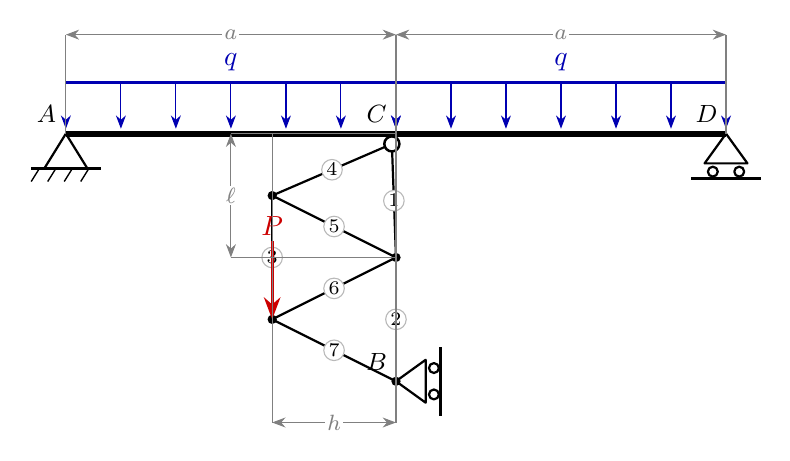
\begin{tikzpicture}[scale=1.048,>=Stealth,line join=round]
  \coordinate (P0) at (0.000,0.000);
  \coordinate (P1) at (4.000,0.000);
  \coordinate (P2) at (8.000,0.000);
  \coordinate (TO1) at (4.000,-1.500);
  \coordinate (TO2) at (4.000,-3.000);
  \coordinate (TU0) at (2.500,-0.750);
  \coordinate (TU1) at (2.500,-2.250);
  \coordinate (CPIN) at (3.950,-0.124);
  \draw[thick] (CPIN) -- (TO1);
  \draw[thick] (TO1) -- (TO2);
  \draw[thick] (TU0) -- (TU1);
  \draw[thick] (CPIN) -- (TU0);
  \draw[thick] (TU0) -- (TO1);
  \draw[thick] (TO1) -- (TU1);
  \draw[thick] (TU1) -- (TO2);
  \draw[line width=2.2pt] (P0) -- (P1);
  \draw[line width=2.2pt] (P1) -- (P2);
  \fill (TO1) circle (1.6pt);
  \fill (TO2) circle (1.6pt);
  \fill (TU0) circle (1.6pt);
  \fill (TU1) circle (1.6pt);
  \draw[fill=white,line width=0.9pt] (CPIN) circle (2.6pt);
  \draw[thick] (0.000,0.000) -- (-0.260,-0.420) -- (0.260,-0.420) -- cycle;
  \draw[line width=1pt] (-0.420,-0.420) -- (0.420,-0.420);
  \draw[line width=0.5pt] (-0.320,-0.420) -- (-0.420,-0.580);
  \draw[line width=0.5pt] (-0.120,-0.420) -- (-0.220,-0.580);
  \draw[line width=0.5pt] (0.080,-0.420) -- (-0.020,-0.580);
  \draw[line width=0.5pt] (0.280,-0.420) -- (0.180,-0.580);
  \draw[thick] (8.000,0.000) -- (7.740,-0.360) -- (8.260,-0.360) -- cycle;
  \draw[thick] (7.840,-0.460) circle (0.06) (8.160,-0.460) circle (0.06);
  \draw[line width=1pt] (7.580,-0.540) -- (8.420,-0.540);
  \draw[thick] (4.000,-3.000) -- (4.360,-3.260) -- (4.360,-2.740) -- cycle;
  \draw[thick] (4.460,-3.160) circle (0.06) (4.460,-2.840) circle (0.06);
  \draw[line width=1pt] (4.540,-3.420) -- (4.540,-2.580);
  \node[circle,fill=white,draw=gray!55,inner sep=0.5pt,font=\scriptsize] at (3.975,-0.812) {1};
  \node[circle,fill=white,draw=gray!55,inner sep=0.5pt,font=\scriptsize] at (4.000,-2.250) {2};
  \node[circle,fill=white,draw=gray!55,inner sep=0.5pt,font=\scriptsize] at (2.500,-1.500) {3};
  \node[circle,fill=white,draw=gray!55,inner sep=0.5pt,font=\scriptsize] at (3.225,-0.437) {4};
  \node[circle,fill=white,draw=gray!55,inner sep=0.5pt,font=\scriptsize] at (3.250,-1.125) {5};
  \node[circle,fill=white,draw=gray!55,inner sep=0.5pt,font=\scriptsize] at (3.250,-1.875) {6};
  \node[circle,fill=white,draw=gray!55,inner sep=0.5pt,font=\scriptsize] at (3.250,-2.625) {7};
  \draw[->,blue!70!black] (0.000,0.620) -- (0.000,0.060);
  \draw[->,blue!70!black] (0.667,0.620) -- (0.667,0.060);
  \draw[->,blue!70!black] (1.333,0.620) -- (1.333,0.060);
  \draw[->,blue!70!black] (2.000,0.620) -- (2.000,0.060);
  \draw[->,blue!70!black] (2.667,0.620) -- (2.667,0.060);
  \draw[->,blue!70!black] (3.333,0.620) -- (3.333,0.060);
  \draw[->,blue!70!black] (4.000,0.620) -- (4.000,0.060);
  \draw[blue!70!black,thick] (0.000,0.620) -- (4.000,0.620);
  \node[blue!70!black] at (2.000,0.870) {$q$};
  \draw[->,blue!70!black] (4.000,0.620) -- (4.000,0.060);
  \draw[->,blue!70!black] (4.667,0.620) -- (4.667,0.060);
  \draw[->,blue!70!black] (5.333,0.620) -- (5.333,0.060);
  \draw[->,blue!70!black] (6.000,0.620) -- (6.000,0.060);
  \draw[->,blue!70!black] (6.667,0.620) -- (6.667,0.060);
  \draw[->,blue!70!black] (7.333,0.620) -- (7.333,0.060);
  \draw[->,blue!70!black] (8.000,0.620) -- (8.000,0.060);
  \draw[blue!70!black,thick] (4.000,0.620) -- (8.000,0.620);
  \node[blue!70!black] at (6.000,0.870) {$q$};
  \draw[->,red!80!black,line width=1.1pt] (2.500,-1.300) -- (2.500,-2.250);
  \node[red!80!black] at (2.500,-1.120) {$P$};
  \draw[thin,gray] (0.000,0.000) -- (0.000,1.200);
  \draw[thin,gray] (4.000,0.000) -- (4.000,1.200);
  \draw[<->,gray] (0.000,1.200) -- (4.000,1.200) node[midway,fill=white,inner sep=0.8pt,font=\footnotesize]{$a$};
  \draw[thin,gray] (4.000,0.000) -- (4.000,1.200);
  \draw[thin,gray] (8.000,0.000) -- (8.000,1.200);
  \draw[<->,gray] (4.000,1.200) -- (8.000,1.200) node[midway,fill=white,inner sep=0.8pt,font=\footnotesize]{$a$};
  \draw[thin,gray] (4.000,0.000) -- (2.000,0.000);
  \draw[thin,gray] (4.000,-1.500) -- (2.000,-1.500);
  \draw[<->,gray] (2.000,0.000) -- (2.000,-1.500) node[midway,fill=white,inner sep=0.8pt,font=\footnotesize]{$\ell$};
  \draw[thin,gray] (4.000,0.000) -- (4.000,-3.500);
  \draw[thin,gray] (2.500,0.000) -- (2.500,-3.500);
  \draw[<->,gray] (4.000,-3.500) -- (2.500,-3.500) node[midway,fill=white,inner sep=0.8pt,font=\footnotesize]{$h$};
  \node[font=\small] at (0.000,0.000) [xshift=-7pt,yshift=7pt] {$A$};
  \node[font=\small] at (4.000,0.000) [xshift=-7pt,yshift=7pt] {$C$};
  \node[font=\small] at (8.000,0.000) [xshift=-7pt,yshift=7pt] {$D$};
  \node[font=\small] at (4.000,-3.000) [xshift=-7pt,yshift=7pt] {$B$};
\end{tikzpicture}
\end{center}
\par\medskip\textbf{1.\ Static determinacy}\par Counting criterion $n=3k-(a+z)$ (bodies $k$, reactions $a$, interaction forces $z$):
\[ n=3k-(a+z)=3\cdot2-(4+2)=0\ \Rightarrow\ \text{statically determinate} \]
\par\medskip\textbf{2.\ Support reactions and hinge forces}\par
$A:\ R_x=6,\ R_y=14$\quad $D:\ R_x=0,\ R_y=14$\quad $B:\ R_x=-6,\ R_y=0$\par $C:\ H_x=-6,\ H_y=-12$
\par\medskip\textbf{3.\ Truss member forces}\par
\begin{center}\renewcommand{\arraystretch}{1.1}\begin{tabular}{c r l}
\toprule
Member & Force $S$ [kN] & Type \\
\midrule
  1 & 9 & tension \\
  2 & 3 & tension \\
  3 & 6 & tension \\
  4 & 6.71 & tension \\
  5 & -6.71 & compression \\
  6 & 6.71 & tension \\
  7 & -6.71 & compression \\
\bottomrule
\end{tabular}\end{center}
\begin{center}
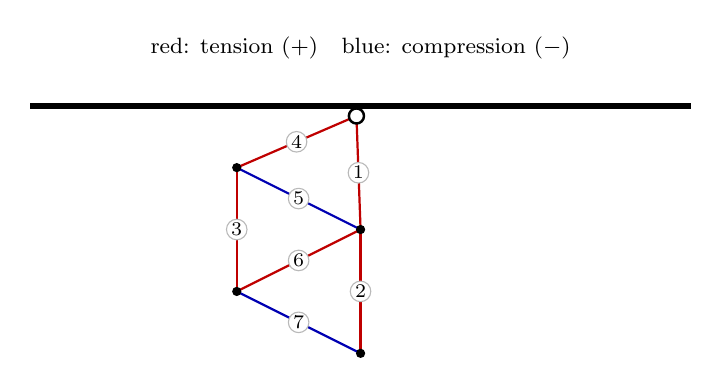
\begin{tikzpicture}[scale=1.048,>=Stealth,line join=round]
  \coordinate (P0) at (0.000,0.000);
  \coordinate (P1) at (4.000,0.000);
  \coordinate (P2) at (8.000,0.000);
  \coordinate (TO1) at (4.000,-1.500);
  \coordinate (TO2) at (4.000,-3.000);
  \coordinate (TU0) at (2.500,-0.750);
  \coordinate (TU1) at (2.500,-2.250);
  \coordinate (CPIN) at (3.950,-0.124);
  \draw[thick,red!75!black] (CPIN) -- (TO1);
  \draw[thick,red!75!black] (TO1) -- (TO2);
  \draw[thick,red!75!black] (TU0) -- (TU1);
  \draw[thick,red!75!black] (CPIN) -- (TU0);
  \draw[thick,blue!70!black] (TU0) -- (TO1);
  \draw[thick,red!75!black] (TO1) -- (TU1);
  \draw[thick,blue!70!black] (TU1) -- (TO2);
  \draw[line width=2pt] (P0) -- (P1);
  \draw[line width=2pt] (P1) -- (P2);
  \fill (TO1) circle (1.6pt);
  \fill (TO2) circle (1.6pt);
  \fill (TU0) circle (1.6pt);
  \fill (TU1) circle (1.6pt);
  \draw[fill=white,line width=0.9pt] (CPIN) circle (2.6pt);
  \node[circle,fill=white,draw=gray!55,inner sep=0.5pt,font=\scriptsize] at (3.975,-0.812) {1};
  \node[circle,fill=white,draw=gray!55,inner sep=0.5pt,font=\scriptsize] at (4.000,-2.250) {2};
  \node[circle,fill=white,draw=gray!55,inner sep=0.5pt,font=\scriptsize] at (2.500,-1.500) {3};
  \node[circle,fill=white,draw=gray!55,inner sep=0.5pt,font=\scriptsize] at (3.225,-0.437) {4};
  \node[circle,fill=white,draw=gray!55,inner sep=0.5pt,font=\scriptsize] at (3.250,-1.125) {5};
  \node[circle,fill=white,draw=gray!55,inner sep=0.5pt,font=\scriptsize] at (3.250,-1.875) {6};
  \node[circle,fill=white,draw=gray!55,inner sep=0.5pt,font=\scriptsize] at (3.250,-2.625) {7};
  \node[font=\footnotesize] at (4.00,0.70) {red: tension $(+)$\quad blue: compression $(-)$};
\end{tikzpicture}
\end{center}
\par\medskip\textbf{4.\ Section-force diagrams of the beams}\par
\begin{center}
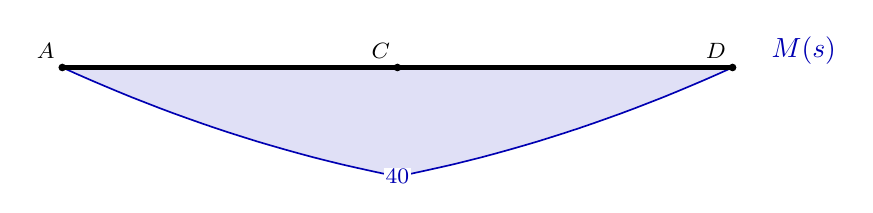
\begin{tikzpicture}[scale=1.064,line join=round]
  \filldraw[fill=blue!70!black!12,draw=blue!70!black,semithick] (0.000,0.000) -- (0.167,-0.075) -- (0.333,-0.148) -- (0.500,-0.219) -- (0.667,-0.289) -- (0.833,-0.357) -- (1.000,-0.422) -- (1.167,-0.487) -- (1.333,-0.549) -- (1.500,-0.609) -- (1.667,-0.668) -- (1.833,-0.725) -- (2.000,-0.780) -- (2.167,-0.833) -- (2.333,-0.885) -- (2.500,-0.934) -- (2.667,-0.982) -- (2.833,-1.028) -- (3.000,-1.073) -- (3.167,-1.115) -- (3.333,-1.156) -- (3.500,-1.194) -- (3.667,-1.231) -- (3.833,-1.267) -- (4.000,-1.300) -- (4.000,-1.300) -- (4.167,-1.267) -- (4.333,-1.231) -- (4.500,-1.194) -- (4.667,-1.156) -- (4.833,-1.115) -- (5.000,-1.073) -- (5.167,-1.028) -- (5.333,-0.982) -- (5.500,-0.934) -- (5.667,-0.885) -- (5.833,-0.833) -- (6.000,-0.780) -- (6.167,-0.725) -- (6.333,-0.668) -- (6.500,-0.609) -- (6.667,-0.549) -- (6.833,-0.487) -- (7.000,-0.422) -- (7.167,-0.357) -- (7.333,-0.289) -- (7.500,-0.219) -- (7.667,-0.148) -- (7.833,-0.075) -- (8.000,0.000) -- (8.000,0.000) -- (7.833,0.000) -- (7.667,0.000) -- (7.500,0.000) -- (7.333,0.000) -- (7.167,0.000) -- (7.000,0.000) -- (6.833,0.000) -- (6.667,0.000) -- (6.500,0.000) -- (6.333,0.000) -- (6.167,0.000) -- (6.000,0.000) -- (5.833,0.000) -- (5.667,0.000) -- (5.500,0.000) -- (5.333,0.000) -- (5.167,0.000) -- (5.000,0.000) -- (4.833,0.000) -- (4.667,0.000) -- (4.500,0.000) -- (4.333,0.000) -- (4.167,0.000) -- (4.000,0.000) -- (4.000,0.000) -- (3.833,0.000) -- (3.667,0.000) -- (3.500,0.000) -- (3.333,0.000) -- (3.167,0.000) -- (3.000,0.000) -- (2.833,0.000) -- (2.667,0.000) -- (2.500,0.000) -- (2.333,0.000) -- (2.167,0.000) -- (2.000,0.000) -- (1.833,0.000) -- (1.667,0.000) -- (1.500,0.000) -- (1.333,0.000) -- (1.167,0.000) -- (1.000,0.000) -- (0.833,0.000) -- (0.667,0.000) -- (0.500,0.000) -- (0.333,0.000) -- (0.167,0.000) -- (0.000,0.000) -- cycle;
  \draw[line width=1.6pt] (0.000,0.000) -- (4.000,0.000) -- (8.000,0.000);
  \node[blue!70!black,font=\footnotesize,fill=white,inner sep=0.5pt] at (4.000,-1.300) {40};
  \fill (0.000,0.000) circle (1.3pt);
  \node[font=\footnotesize] at (0.000,0.000) [xshift=-6pt,yshift=6pt] {$A$};
  \fill (4.000,0.000) circle (1.3pt);
  \node[font=\footnotesize] at (4.000,0.000) [xshift=-6pt,yshift=6pt] {$C$};
  \fill (8.000,0.000) circle (1.3pt);
  \node[font=\footnotesize] at (8.000,0.000) [xshift=-6pt,yshift=6pt] {$D$};
  \node[blue!70!black,right] at (8.35,0.20) {$M(s)$};
\end{tikzpicture}\\[5pt]
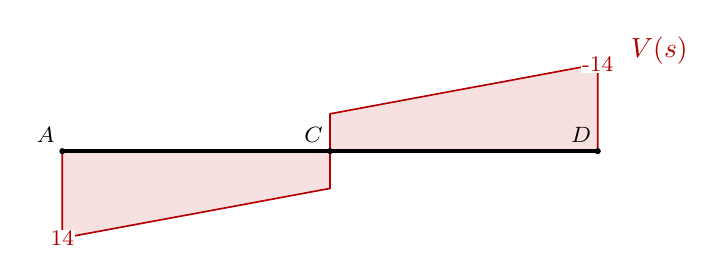
\begin{tikzpicture}[scale=0.850,line join=round]
  \filldraw[fill=red!70!black!12,draw=red!70!black,semithick] (0.000,-1.300) -- (0.167,-1.269) -- (0.333,-1.238) -- (0.500,-1.207) -- (0.667,-1.176) -- (0.833,-1.145) -- (1.000,-1.114) -- (1.167,-1.083) -- (1.333,-1.052) -- (1.500,-1.021) -- (1.667,-0.990) -- (1.833,-0.960) -- (2.000,-0.929) -- (2.167,-0.898) -- (2.333,-0.867) -- (2.500,-0.836) -- (2.667,-0.805) -- (2.833,-0.774) -- (3.000,-0.743) -- (3.167,-0.712) -- (3.333,-0.681) -- (3.500,-0.650) -- (3.667,-0.619) -- (3.833,-0.588) -- (4.000,-0.557) -- (4.000,0.557) -- (4.167,0.588) -- (4.333,0.619) -- (4.500,0.650) -- (4.667,0.681) -- (4.833,0.712) -- (5.000,0.743) -- (5.167,0.774) -- (5.333,0.805) -- (5.500,0.836) -- (5.667,0.867) -- (5.833,0.898) -- (6.000,0.929) -- (6.167,0.960) -- (6.333,0.990) -- (6.500,1.021) -- (6.667,1.052) -- (6.833,1.083) -- (7.000,1.114) -- (7.167,1.145) -- (7.333,1.176) -- (7.500,1.207) -- (7.667,1.238) -- (7.833,1.269) -- (8.000,1.300) -- (8.000,0.000) -- (7.833,0.000) -- (7.667,0.000) -- (7.500,0.000) -- (7.333,0.000) -- (7.167,0.000) -- (7.000,0.000) -- (6.833,0.000) -- (6.667,0.000) -- (6.500,0.000) -- (6.333,0.000) -- (6.167,0.000) -- (6.000,0.000) -- (5.833,0.000) -- (5.667,0.000) -- (5.500,0.000) -- (5.333,0.000) -- (5.167,0.000) -- (5.000,0.000) -- (4.833,0.000) -- (4.667,0.000) -- (4.500,0.000) -- (4.333,0.000) -- (4.167,0.000) -- (4.000,0.000) -- (4.000,0.000) -- (3.833,0.000) -- (3.667,0.000) -- (3.500,0.000) -- (3.333,0.000) -- (3.167,0.000) -- (3.000,0.000) -- (2.833,0.000) -- (2.667,0.000) -- (2.500,0.000) -- (2.333,0.000) -- (2.167,0.000) -- (2.000,0.000) -- (1.833,0.000) -- (1.667,0.000) -- (1.500,0.000) -- (1.333,0.000) -- (1.167,0.000) -- (1.000,0.000) -- (0.833,0.000) -- (0.667,0.000) -- (0.500,0.000) -- (0.333,0.000) -- (0.167,0.000) -- (0.000,0.000) -- cycle;
  \draw[line width=1.6pt] (0.000,0.000) -- (4.000,0.000) -- (8.000,0.000);
  \node[red!70!black,font=\footnotesize,fill=white,inner sep=0.5pt] at (0.000,-1.300) {14};
  \node[red!70!black,font=\footnotesize,fill=white,inner sep=0.5pt] at (8.000,1.300) {-14};
  \fill (0.000,0.000) circle (1.3pt);
  \node[font=\footnotesize] at (0.000,0.000) [xshift=-6pt,yshift=6pt] {$A$};
  \fill (4.000,0.000) circle (1.3pt);
  \node[font=\footnotesize] at (4.000,0.000) [xshift=-6pt,yshift=6pt] {$C$};
  \fill (8.000,0.000) circle (1.3pt);
  \node[font=\footnotesize] at (8.000,0.000) [xshift=-6pt,yshift=6pt] {$D$};
  \node[red!70!black,right] at (8.35,1.50) {$V(s)$};
\end{tikzpicture}\\[5pt]
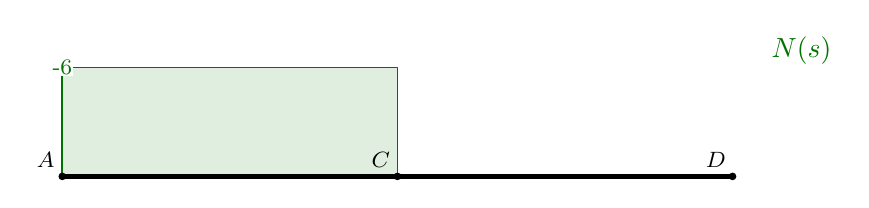
\begin{tikzpicture}[scale=1.064,line join=round]
  \filldraw[fill=green!45!black!12,draw=green!45!black,semithick] (0.000,1.300) -- (0.167,1.300) -- (0.333,1.300) -- (0.500,1.300) -- (0.667,1.300) -- (0.833,1.300) -- (1.000,1.300) -- (1.167,1.300) -- (1.333,1.300) -- (1.500,1.300) -- (1.667,1.300) -- (1.833,1.300) -- (2.000,1.300) -- (2.167,1.300) -- (2.333,1.300) -- (2.500,1.300) -- (2.667,1.300) -- (2.833,1.300) -- (3.000,1.300) -- (3.167,1.300) -- (3.333,1.300) -- (3.500,1.300) -- (3.667,1.300) -- (3.833,1.300) -- (4.000,1.300) -- (4.000,0.000) -- (4.167,0.000) -- (4.333,0.000) -- (4.500,0.000) -- (4.667,0.000) -- (4.833,0.000) -- (5.000,0.000) -- (5.167,0.000) -- (5.333,0.000) -- (5.500,0.000) -- (5.667,0.000) -- (5.833,0.000) -- (6.000,0.000) -- (6.167,0.000) -- (6.333,0.000) -- (6.500,0.000) -- (6.667,0.000) -- (6.833,0.000) -- (7.000,0.000) -- (7.167,0.000) -- (7.333,0.000) -- (7.500,0.000) -- (7.667,0.000) -- (7.833,0.000) -- (8.000,0.000) -- (8.000,0.000) -- (7.833,0.000) -- (7.667,0.000) -- (7.500,0.000) -- (7.333,0.000) -- (7.167,0.000) -- (7.000,0.000) -- (6.833,0.000) -- (6.667,0.000) -- (6.500,0.000) -- (6.333,0.000) -- (6.167,0.000) -- (6.000,0.000) -- (5.833,0.000) -- (5.667,0.000) -- (5.500,0.000) -- (5.333,0.000) -- (5.167,0.000) -- (5.000,0.000) -- (4.833,0.000) -- (4.667,0.000) -- (4.500,0.000) -- (4.333,0.000) -- (4.167,0.000) -- (4.000,0.000) -- (4.000,0.000) -- (3.833,0.000) -- (3.667,0.000) -- (3.500,0.000) -- (3.333,0.000) -- (3.167,0.000) -- (3.000,0.000) -- (2.833,0.000) -- (2.667,0.000) -- (2.500,0.000) -- (2.333,0.000) -- (2.167,0.000) -- (2.000,0.000) -- (1.833,0.000) -- (1.667,0.000) -- (1.500,0.000) -- (1.333,0.000) -- (1.167,0.000) -- (1.000,0.000) -- (0.833,0.000) -- (0.667,0.000) -- (0.500,0.000) -- (0.333,0.000) -- (0.167,0.000) -- (0.000,0.000) -- cycle;
  \draw[line width=1.6pt] (0.000,0.000) -- (4.000,0.000) -- (8.000,0.000);
  \node[green!45!black,font=\footnotesize,fill=white,inner sep=0.5pt] at (0.000,1.300) {-6};
  \fill (0.000,0.000) circle (1.3pt);
  \node[font=\footnotesize] at (0.000,0.000) [xshift=-6pt,yshift=6pt] {$A$};
  \fill (4.000,0.000) circle (1.3pt);
  \node[font=\footnotesize] at (4.000,0.000) [xshift=-6pt,yshift=6pt] {$C$};
  \fill (8.000,0.000) circle (1.3pt);
  \node[font=\footnotesize] at (8.000,0.000) [xshift=-6pt,yshift=6pt] {$D$};
  \node[green!45!black,right] at (8.35,1.50) {$N(s)$};
\end{tikzpicture}\\[10pt]
\end{center}
\end{document}